\documentclass[a4paper]{article}
\usepackage[utf8]{inputenc}
\usepackage[IL2]{fontenc}
\usepackage[czech]{babel}
\usepackage[left=3cm, text={15cm,24cm}, top=3cm]{geometry}

\usepackage{graphicx}
\usepackage[export]{adjustbox}
\usepackage{listings}
\usepackage{verbatim}
\usepackage[colorlinks=true]{hyperref}
\usepackage{array,tabularx}

\newenvironment{conditions*}
  {\par\vspace{\abovedisplayskip}\noindent
   \tabularx{\columnwidth}{>{$}l<{$} @{\ : } >{\raggedright\arraybackslash}X}}
  {\endtabularx\par\vspace{\belowdisplayskip}}

\begin{document}
\thispagestyle{empty}
\begin{center}
\LARGE
\textsc{Vysoké učení technické v Brně \\
Fakulta informačních technologií}\\
\vspace{\stretch{0.15}}

\includegraphics[width = 8 cm]{pic/FIT_barevne_CMYK_CZ.eps}
\vspace{\stretch{0.2}}

\LARGE
\textbf{Umělá inteligence a strojové učení}\\
Umělá inteligence pro Válku kostek \\
\vspace {\stretch{0.65}}

\end{center}
Jan Chaloupka (xchalo16) - vedoucí týmu \\
Michal Krůl (xkrulm00) \\
Jan Láncoš (xlanco00)
\hfill
\today

\newpage
\setcounter{page}{1}

\section{Úvod}

Cílem projektu bylo implementovat umělou inteligenci (dále AI) pro hru Dice Wars. Umělá inteligence by měla být schopna hrát tuto hru, založenou z velké části na náhodě. Její kvalita by měla následně být hodnocena schopností porážet ostatní umělé inteligence, které již byly ke hře vytvořeny.

\section{Vytvořená umělá inteligence}

Hráč ovládaný naší AI pracuje na principu algoritmu expectiminimax, který je rozšířený pro hru více hráčů (také označován jako Max\textsuperscript{N}, více v sekci \ref{sec:maxn}). Algoritmus je nastavený na prohledávání stavového prostoru do hloubky osmi vrstev (důvody výběru prohledávání právě do hloubky 8 viz sekce \ref{sec:testhloubky}). Při počtu čtyř hráčů tedy simuluje dva celé nadcházející tahy hry.

\subsection{Heuristická funkce}

Algoritmus Max\textsuperscript{N} využívá k ohodnocení dvě heuristiky -- \textbf{ohodnocení současného stavu herního pole} pro aktuálního hráče a \textbf{ohodnocení konkrétního útoku}.

\subsubsection*{Heuristika současného stavu herního pole}
\label{sec:hpole}
Jako metriku ohodnocení současného stavu hry je použito současné skóre hráče -- tedy součet polí v největším souvislém regionu, který hráč vlastní. 

\subsubsection*{Heuristika bitvy}
\label{sec:hbitvy}
Heuristická funkce ohodnocení bitvy bere v potaz ohodnocení stavu hry po vyhrané bitvě a stav hry po prohrané bitvě. Tyto koeficienty jsou vynásobeny pravděpodobností, že dané situace nastanou, a následně jsou od sebe odečteny. Výsledkem je celkové ohodnocení bitvy vyjadřující potenciální zisk po jejím iniciování. Před odečtením těchto složek je však první z koeficientů ještě vynásoben pravděpodobností vyjadřující šanci na udržení dobytého pole. Pravděpodobnost udržení pole je součinem pravděpodobností každého úspěšně ubráněného napadení daného pole, ke kterému by teoreticky za současného stavu hry mohlo dojít. Matematicky lze ohodnocení vyjádřit jako:
\[
ohodnoceni\ bitvy = \Big( prob(succ) \times field(succ) \times prob_{hold}(succ)\Big) - \Big( prob(fail) \times field(fail)\Big)
\]
kde
\begin{conditions*}
 prob(succ)  & pravděpodobnost úspěšného útoku\\
 field(succ) & ohodnocení stavu herního pole pro útočníka při úspěšném útoku\\
 prob_{hold}(succ)  & pravděpodobnost udržení nově získaného pole\\
 prob(fail)  & pravděpodobnost neúspěšného útoku\\
 field(fail) & ohodnocení stavu herního pole pro útočníka při neúspěšném útoku
\end{conditions*}

Platí tedy, že čím vyšší ohodnocení, tím je tah výhodnější. Záporné ohodnocení bitvy je obecně považováno za nevýhodné a AI preferuje ukončit tah v okamžiku, kdy jsou všechny dostupné akce ohodnoceny záporně. Tah ukončí také po pěti po sobě jdoucích akcích z důvodu časového omezení. Po každé provedené akci je situace vyhodnocena znovu a AI tedy může provést sekvenci útoků do určitého území.

\subsection{Algoritmus Max\textsuperscript{N} (prohledávání stavového prostoru)}
\label{sec:maxn}

Algoritmus expectiminimax vyjadřuje ohodnocení hry jediným číslem, které lze minimalizovat, nebo maximalizovat. Je tedy omezen pro dva hráče. V našem případě je tedy třeba použít jeho modifikaci zvanou algoritmus Max\textsuperscript{N}, ve které má každý hráč své vlastní ohodnocení hry a všichni se to svoje snaží maximalizovat.

Algoritmus funguje na sestavení stromu akcí a reakcí protihráčů, kde každé patro reprezentuje možné tahy jednoho hráče. Strom je sestaven jako výčet všech validních bitev, které má daný hráč po předchozím tahu jiného hráče k dispozici. Vzhledem ke stavové explozi jsou všechny možné bitvy předem filtrovány. Filtrování začíná ohodnocením bitev heuristickou funkcí (viz \ref{sec:hbitvy}) a zavržením všech bitev, které se jeví jako nevýhodné (ohodnocení $<0$). Výjimku tvoří bitvy z políčka, na kterém je maximální počet kostek -- ty nejsou filtrovány a berou se vždy jako výhodné. Nakonec se vezme v úvahu pouze určitý maximální počet nejlépe ohodnocených bitev (při testování bylo zjištěno, že 5 nejlepších bitev stačí k dobrému ohodnocení).

Po dosažení předem určené poslední úrovně stromu se vyhodnotí současný stav hry pro všechny hráče (hodnocení probíhá heuristikou funkcí ohodnocení stavu herního pole, viz \ref{sec:hpole}). Každý hráč po vyhodnocení vyfiltrovaných bitev vybere nejlepší z nich a potenciálně nejlepší hodnocení deleguje do vyšších pater. Hráč na vyšší úrovni započítá pravděpodobný stav hry po provedení svých tahů s ohledem na protitahy protihráčů a provádí stejnou akci, dokud se informace nedostane na vrchol stromu a AI provádějící simulaci tedy zjistí objektivně nejlepší tah, který momentálně může provést.

Algoritmus předpokládá, že protihráči hrají stejným způsobem a využívají stejnou heuristickou funkci.

\section{Postup vylepšování AI}
\label{sec:vylepsovaniai}

Původní heuristika byla navržena tak, že ohodnocení bitvy bylo založeno na výsledném skóre hráče v případě úspěšného útoku, počtu polí, které je potenciálně možné dál napadnout z dobytého území a počtu polí, které by mohly být naopak napadeny protihráčem. Tato heuristika byla nakonec zavržena, neboť později výše popsaná jednodušší heuristika vykazovala lepší výsledky a bylo náročné mnoho faktorů původní heuristiky vhodně nastavit.

Pro fungování algoritmu Max\textsuperscript{N} bylo potřeba simulovat přidávání kostek hráčům na konci kola. Protože přidávání je určováno náhodně, nelze přesně určit, jaký bude stav hry před dalším zanořením algoritmu. Byl tedy navrhnut způsob simulující nejhorší možnost rozvržení kostek při každém přidělování kostek v rámci algoritmu z pohledu implementované AI. Jako nejhorší možnost bylo určeno navršení získaných kostek do polí, které nesdílely hranici s žádným polem protihráčů. Jako nejhorší možnost při přidělování kostek protihráčům z pohledu implementované AI bylo určeno rovnoměrné rozvržení kostek mezi hraniční pole jejich území. V principu tedy šlo o okamžité navýšení útočné kapacity všech protihráčů. Tento způsob simulace rozdělování kostek a tedy vycházení z nejhorší možné eventuality však vykazoval horší výsledky, než když bylo rozdělení kostek simulováno náhodně a proto nebyl použit.

Obecně je náhodné rozdělení kostek ve hře velkým problémem při předvídání stavu hry několik tahů dopředu. Pokud je snaha vyvarovat se pouhému slepému procházení všech možností (kterých je ve hře s průměrně třiceti poli a až 8 kostkami na jednom poli velmi mnoho), je pravděpodobné, že rozložení zvolené při zanořování algoritmu nebude odpovídající a tím pádem předvídání tahů protihráčů ztrácí na relevanci. Testováním bylo zjištěno, že sice statisticky pracuje AI líp, když se snaží tímto způsobem předvídat tahy protihráčů, než když se soustředí pouze na současný stav hry, ovšem při hlubším zanoření algoritmu se již akumuluje vliv náhody a AI opět vykazuje horší výsledky.

Každá verze AI byla podrobena testování. Testování proběhlo na turnajích s ostatními AI definovanými v podmínkách hodnocení. Testovalo se na turnajích především s hodnotou opakovaní $n=100$, s různou hloubkou prohledávání našeho algoritmu Max\textsuperscript{N} a různým seedem. Z výsledků těchto turnajů, kde bylo především bráno v potaz procento vyhraných her (ale také byl brán v potaz trend úspěšnosti s přibývajícím počtem her), byly odvozovány závěry, o kvalitě vytvořené AI.

\subsection{Zjištění optimální hloubky prohledávání}
\label{sec:testhloubky}
Testováním bylo zjištěno, jaká hloubka prohledávání je pro naši AI optimální. Testování probíhalo spuštěním stejného turnaje pro hloubku prohledávání 1, 4, 8 a 12\footnote{Hloubka prohledávání je počet tahů. Tedy pokud jsou ve hře 4 hráči a hloubka prohledávání je 4, odehraje se celé kolo. U hloubky 1 se nebere v potaz žádná reakce protihráčů na zvolený tah.}. Takto bylo odehráno 16 turnajů ($4\times4$) a výsledná procentuální úspěšnost každého turnaje byla zanesena do grafu, viz obrázek \ref{graf:vyhryhloubka}. Při zprůměrování všech turnajů za danou hloubku je vidět, že počet výher naší AI stoupá až do hloubky 8. Dále s větší hloubkou úspěšnost začne výrazně klesat. Příčinou může být akumulující se chyba odhadu hry (pravděpodobně díky náhodnému rozdělení kostek po každém tahu) nebo špatně zvolená heuristická funkce. Každopádně se v našem případě jako nejlepší počet iterací jeví právě 8.

\begin{figure}[htb]
	\centering
	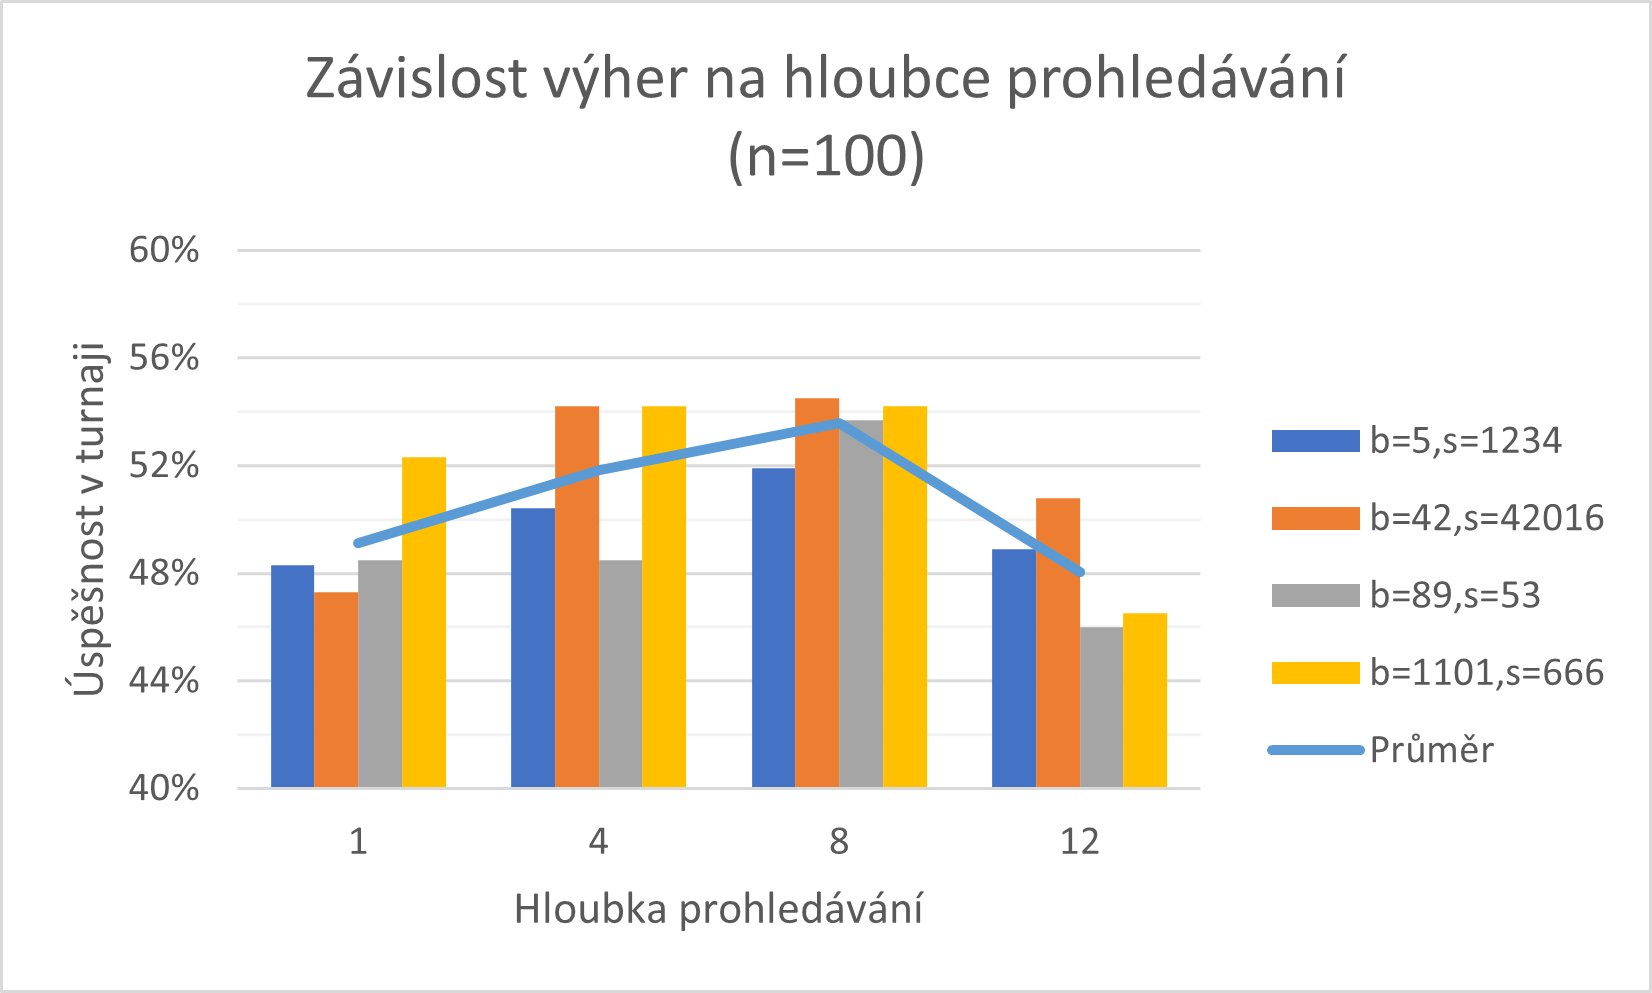
\includegraphics[height=7cm]{pic/vyhry_hloubka_graf.png}
	\caption{Graf znázorňující závislost výher v turnaji na hloubce prohledávání stavů našeho Max\textsuperscript{N} algoritmu.}
	\label{graf:vyhryhloubka}
\end{figure}

Aby naše AI nebyla příliš pomalá, byl vybrán jeden testovací turnaj u kterého proběhlo měření celkového času turnaje. Výsledné hodnoty jsou zaneseny do grafu na obrázku \ref{graf:cashloubka}. Na tomto grafu je vidět exponenciální růst stráveného času dle hloubky procházení. I přes narůstající časovou náročnost bylo 12 iterací pořád dostatečně rychlé pro časový limit stanovený hrou. Jedno volání metody pro tah AI při hloubce 8 trvalo na procesoru Intel Xeon E3-1270v3 řádově desítky milisekund. I přes to je pro jistotu v implementaci podmínka, kdy při nedostatečném času se provádí pouze 4 nebo 1 iterace. Při testování na školním serveru merlin ke snížení nedošlo a počítalo se vždy s hloubkou 8.

\begin{figure}[htb]
	\centering
	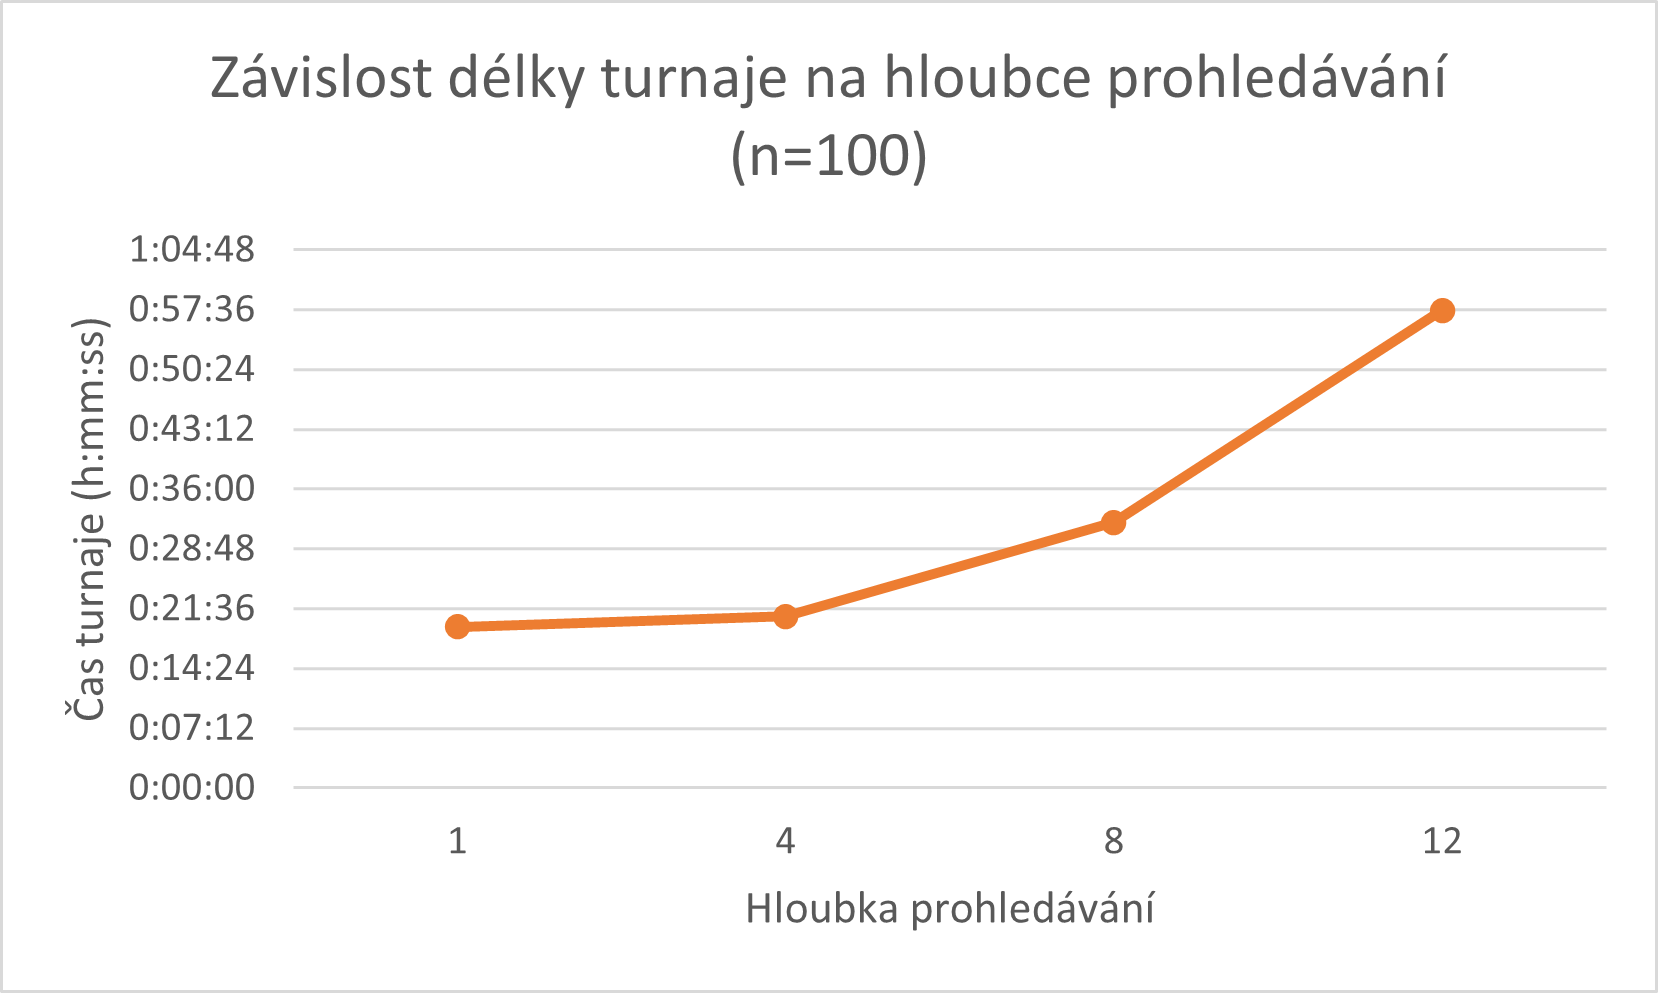
\includegraphics[height=7cm]{pic/cas_hloubka_graf.png}
	\caption{Graf znázorňující exponenciální časovou náročnost v závislosti na hloubce prohledávání stavového prostoru našeho Max\textsuperscript{N} algoritmu.}
	\label{graf:cashloubka}
\end{figure}

\section{Implementace}

AI je implementována ve třech souborech jazyka Python. V souboru \texttt{main.py} je implementována třída AI, která představuje umělou inteligenci jako takovou. Při její konstrukci je volán konstruktor třídy MaxN, která je implementována v souboru \texttt{maxn.py}. Funkce, které zajišťují výpočet heuristiky, simulace bitev a přidávání kostek jsou implementovány v souboru \texttt{utils.py}. V kódu se využívá některých existujících funkcí z modulu \texttt{dicewars.ai.utils} -- jde například o funkce pro zjištění pravděpodobnosti útoku nebo získání všech možných bitev.

\subsection{Popis jedné akce AI}

Volaná metoda \texttt{ai\_turn()} je hlavním vstupem pro rozhodování o následujícím tahu. V závislosti na dostupném čase dynamicky mění hloubku prohledávání a dále volá metodu instance třídy MaxN, která nalezne nejlepší možný tah a podle toho je buď zaslán příkaz \texttt{BattleComand} nebo \texttt{EndTurnCommand}. Tato metoda ze třídy \texttt{MaxN} s názvem \texttt{get\_best\_move()} je pouze spouštějící funkcí pro rekurzi algoritmu Max\textsuperscript{N}. Hlavní rekurzivní funkce má název \texttt{\_\_make\_turn()}. Ta při svém běhu provede jedno zanoření algoritmu, ohodnotí všechny možné tahy heuristickou funkcí (\texttt{battle\_heuristic()}) a před dalším rekurzivním voláním sebe sama provede simulaci bitvy (funkce \texttt{simulate\_battle()}) a rozdělení kostek (funkce \texttt{add\_dices\_to\_player()}).
 
\section{Možné vylepšení}

Ačkoliv jsme s výkonem naší AI spokojení, rozhodně není dokonalá. Na následujících řádcích tedy navrhujeme možnosti, jak by šlo v budoucnu vylepšit její chování a zajistit ještě vyšší poměr výher.

\subsection{Náhodnost při doplňování kostek}

Jak již bylo zmíněno v sekci \ref{sec:vylepsovaniai}, simulace přidávání kostek na konci tahu funguje na principu náhodu a z toho důvodu je velmi nepředvídatelná. Je tedy téměř nemožné odhadnout a přesně napodobit stav hry v předvídání protitahů oponentů a chyba se s každým dalším tahem akumuluje. Přidávání kostek náhodně, stejně jako to dělá hra, však spíše stav hry nevystihne, než vystihne. Přesto se však tento způsob projevil jako efektivnější, než přidávání kostek nesimulovat vůbec, nebo se pokoušet o simulaci nejhorší možné eventuality. Tento způsob však stále není ideální, a faktor náhody v rozhodování AI ji činí o to víc nekonzistentní. Je tedy vhodné, pokud by to vůbec bylo možné, náhodnost z rozhodování odstranit.  

\subsection{Ochota riskovat pro možnost vyššího zisku}

AI momentálně není schopna identifikovat možnost podstoupit bitvu s nízkou odměnou za účelem získání možnosti pokusit se o bitvu s odměnou vysokou. Hodnotí pouze pole ve svém blízkém okolí a v rámci tahu plně nevyužívá potenciálu řetězení akcí k tomuto účelu. Bylo by možné a vhodné implementovat schopnost odhalení snadno napadnutelných nebo klíčových polí ve větší vzdálenosti, ke kterým se vyplatí se probojovat i za cenu nízké odměny či případně většího rizika. U těchto útočných sekvencí by bylo třeba počítat s násobením pravděpodobností úspěchu. Tyto akce by tedy vždy byly riskantní, ale velmi lukrativní. 

\subsection{Snaha o propojení dvou území}

AI se snaží co nejvíce rozšířit své území dobýváním libovolných okolních polí. Mohlo by být ovšem vhodné, aby si uvědomovala všechny regiony, které vlastní, a snažila se o jejich propojení. Momentálně k tomuto dochází pouze v okamžiku, kdy území odděluje pouze jedno cizí pole. AI v tom okamžiku heuristickou funkcí vyhodnotí, že by došlo k masivnímu navýšení velikostí skóre, neboť by došlo ke skokovému zvětšení největšího regionu.

Vědomé snahy propojit území i v ostatních okamžicích by mohlo být dosaženo prohledáváním do šířky z největšího regionu (pokud bereme hrací pole jako neorientovaný graf), nalezení nejkratší cesty mezi dvěma regiony a následné preferování útoků, které by délku této cesty snižovaly.

\subsection{Nevyřazovat potenciální spojence}
Ze strategického hlediska je rozumné udržovat své oponenty zaměstnané mezi sebou a pokud možno nedovolit jednomu asimilovat druhého a nabrat tím sílu. Dobrá heuristika by tedy byla schopna určit, kterého oponenta je v daný moment vhodnější napadnout. Vzhledem k tomu, že oponenti hrají racionálně a nebudou se tedy mstít, a že nemohou přímo a spolehlivě ovlivnit svoji útočnou kapacitu, je vždy vhodnější napadnout silnějšího protivníka, jsou-li obě potenciální bitvy jinak heuristikou hodnoceny ekvivalentně. Stejně velké území ovládané dvěma hráči je vždy slabší, než pokud je na něm pouze jeden hráč. Je tedy v našem zájmu slabšího oponenta nevyřadit zbytečně.

Jinou situací však je, pokud se například nachází naše území mezi dvěma oponenty a oni spolu nesdílejí žádné hranice. To je přesně opačná situace a je proto třeba naopak silně soustředit útočnou kapacitu jedním směrem a jednoho z oponentů vyřadit definitivně. Je-li tedy nějaké pole schopno napadnout oba oponenty, AI by měla preferovat útok na oponenta, kterého jde napadnout i z jiného pole. V tomto případě je snaha oponenty udržet stejně silné kontraproduktivní. 

Tohoto by šlo například dosáhnout vhodným zhodnocením poměru množství hranic, které mezi sebou sdílejí oponenti, a které s nimi všemi sdílí námi implementovaná AI. Je-li mnoho hranic mezi naší AI a jejími oponenty a málo hranic mezi oponenty samými, není třeba se zabývat srovnáváním sil. Pokud je však mnoho hranic mezi oponenty, je vhodné v případě volby preferovat napadení silnějšího protivníka a tím pádem srovnání sil mezi nimi.
 
\vfill


\begin{thebibliography}{9}
\bibitem{maxn:stacko} 
Extending minimax algorithm for multiple opponents. \textit{Stack Overflow} [online]. 2020 [cit.~27.12.2020]. Dostupné z: \url{https://stackoverflow.com/a/63609301/3430085}
\bibitem{maxn} 
LUCKHARDT, Carol A a IRANI, Keki B. \textit{AN ALGORITHMIC SOLUTION OF N-PERSON GAMES} [online]. Fifth National Conference on Artificial Intelligence. AAAI Press, 1986 [cit.~27.12.2020]. Dostupné z: \url{https://www.aaai.org/Papers/AAAI/1986/AAAI86-025.pdf}
\end{thebibliography}

\end{document}
